\subsection{ASAP-HSQC excitation delay}
\label{subsec:poise__asaphsqc}

The next example of the ASAP-HSQC experiment\autocite{SchulzeSunninghausen2014JACS,SchulzeSunninghausen2017JMR,Koos2019JMR,Becker2019JMR} continues to illustrate how custom cost functions in POISE can be used to carry out a variety of optimisations.
In the ASAP-HSQC experiment (\cref{fig:asaphsqc_pulseq}), a HSQC spectrum is recorded using only \carbon{}--bound proton magnetisation, and the \carbont{}--bound (`bulk') proton magnetisation is returned to the equilibrium $+z$ axis (i.e.\ the $I_z$ state).
In this way, instead of having a conventional recovery delay, the \carbon{}--\proton{} magnetisation can be directly replenished using isotropic mixing, which causes transfer of $z$-magnetisation from bulk protons.
The elision of the recovery delay from the sequence thus leads to significantly shorter experiment durations: in one of the more extreme examples, a HSQC spectrum could be recorded within 7 seconds.
This separation of different `magnetisation pools' is conceptually very similar to that in NOAH experiments, and in anticipation of that, I use the notation \magn{C} and \magnnot{C} to represent magnetisation belonging to protons coupled and not coupled to \carbon{} respectively.

\begin{figure}[htb]
    \centering
    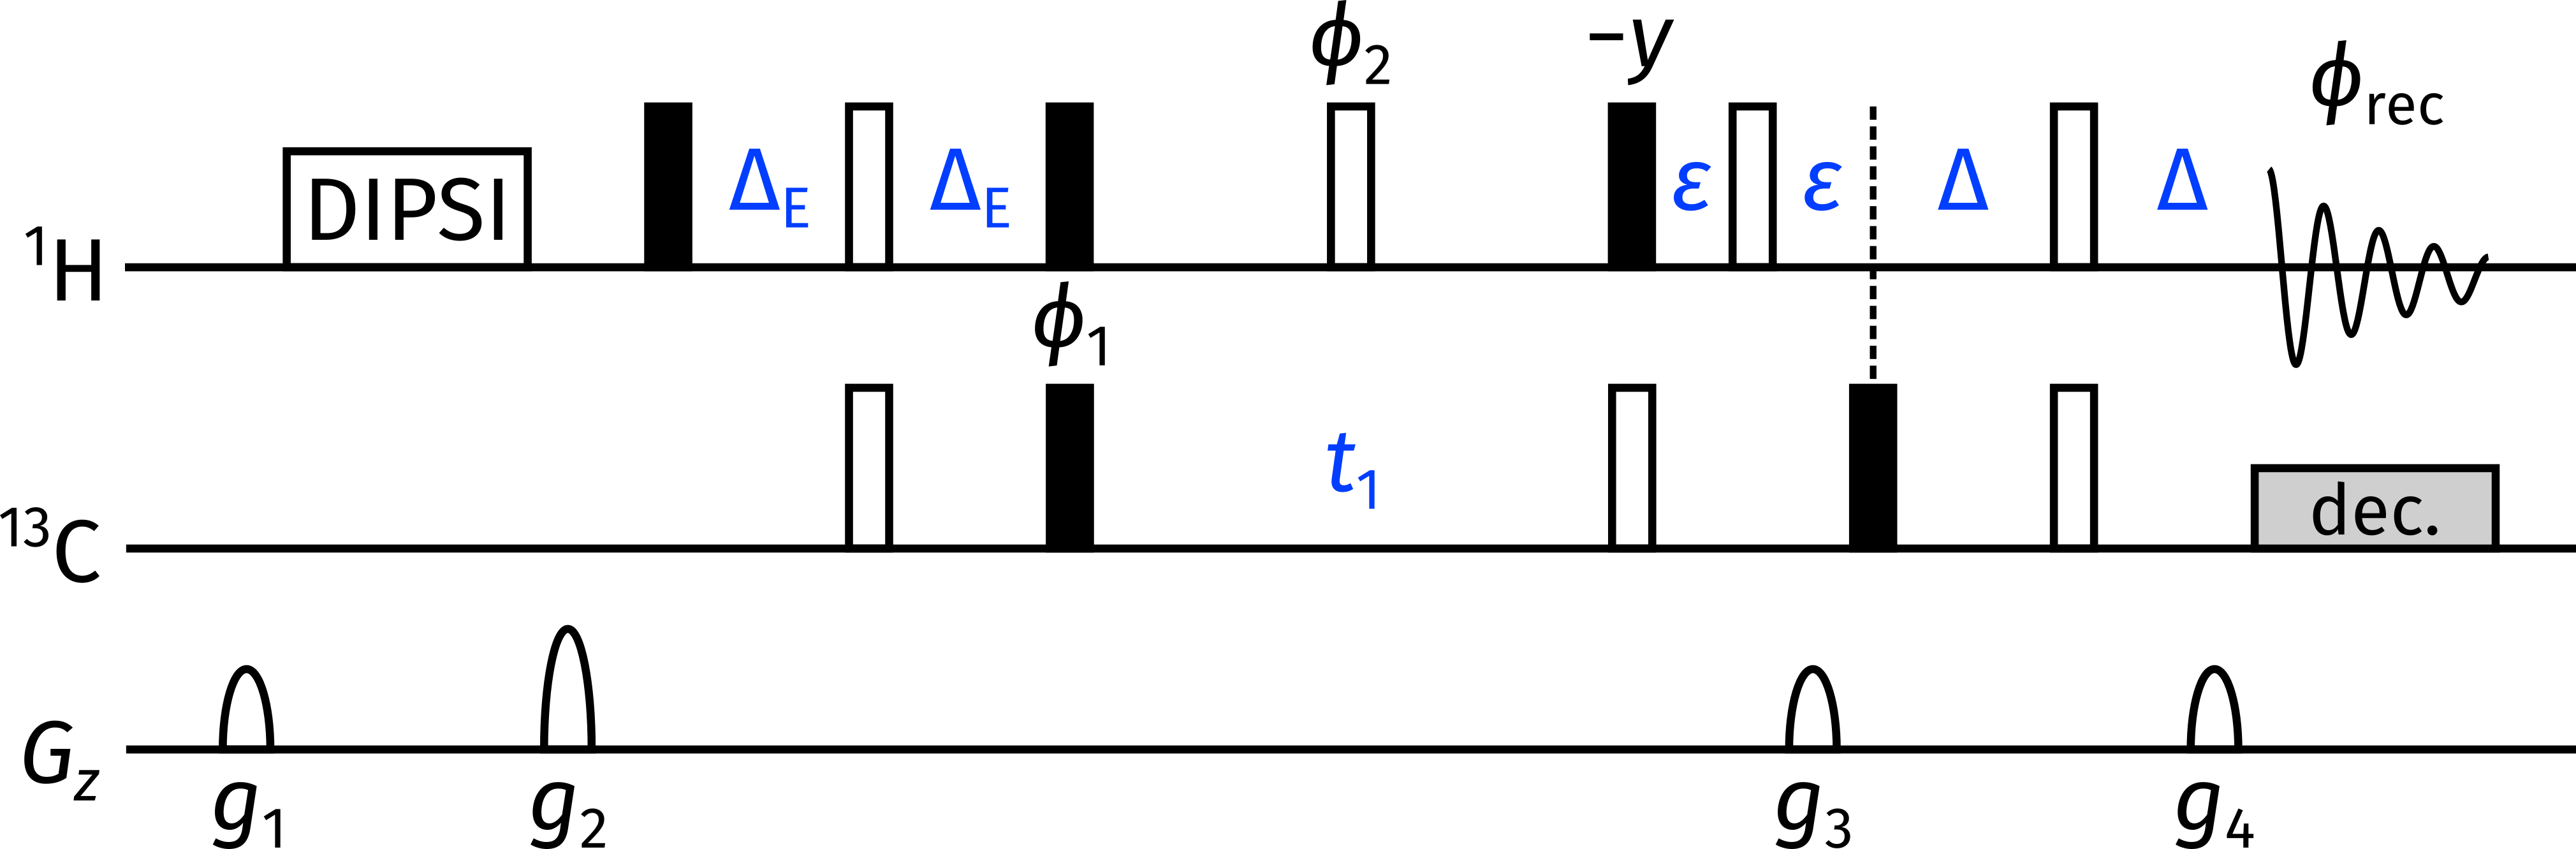
\includegraphics[]{pp/poise/asaphsqc.png}%
    \caption[ASAP-HSQC pulse sequence]{
        ASAP-HSQC pulse sequence.
        Phase cycling is performed using $\phi_1 = (x, -x)$, $\phi_2 = (x, x, -x, -x)$, and $\phi_\text{rec} = (x, -x, x, -x)$.
        Gradient amplitudes are as follows: $g_1 = 33\%$, $g_2 = 43\%$, and for echo--antiecho selection, $(g_3, g_4) = (59.9\%, 80\%)$ and $(63.9\%, 80\%)$ respectively.
        The delay $\Delta$ is set to $1/(4 \cdot \oneJ{CH})$; the delay $\Delta_\text{E}$ was optimised as described in the text.
        The BIBOP, BEBOP, and BURBOP optimal control pulses\autocite{Kobzar2004JMR,Kobzar2008JMR,Kobzar2012JMR} were used for \proton{} \ang{180} pulses and all \carbon{} pulses; for more details, refer to the original paper by Luy and coworkers\autocite{SchulzeSunninghausen2014JACS}.
    }
    \label{fig:asaphsqc_pulseq}
\end{figure}

By modifying the length of the delay $\Delta_\text{E}$ in the initial INEPT block, it is possible to adjust the proportion of the \magn{C} magnetisation excited during the sequence: the remainder is stored along $z$.
This means that the signal is decreased by a factor of $\sin\theta_\text{eff}$ (where $\theta_\text{eff}$ is an effective flip angle), but means that on the next scan or increment, there is a larger pool of \magn{C} magnetisation to start from.
The combination of these factors means that there is an optimum $\Delta_\text{E}$ which yields the greatest steady-state signal.
(Notice that this is entirely analogous to the Ernst angle previously discussed in \cref{subsec:poise__ernst}.)
The delay $\Delta_\text{E}$ is related to the effective flip angle, $\theta_\text{eff}$, through
\begin{equation}
    \label{eq:asaphsqc_ernst_angle}
    \theta_\text{eff} = 2\pi J \Delta_\text{E}.
\end{equation}
where $J$ is here short for $\oneJ{CH}$.
Equivalently, we can define an `effective J-coupling', $J_\text{eff}$ for which the excitation is optimised:
\begin{equation}
    \label{eq:asaphsqc_j_eff}
    \Delta_\text{E} = \frac{1}{4 J_\text{eff}} \quad\Longleftrightarrow\quad J_\text{eff} = \frac{\pi J}{2\theta_\text{eff}}.
\end{equation}


\subsubsection{Optimisation setup}

Given the analysis above, it is extraordinarily easy to set up the optimisation: the parameter being optimised is $J_\text{eff}$, and the initial point chosen is simply $\oneJ{CH}$ (to be precise, a `compromise' $\oneJ{CH}$ value of \qty{150}{\Hz}).
Although generally it is not a good idea to use a 2D experiment as part of the FE, in this specific case it is acceptable because the ASAP-HSQC has such a short running time.
In this case, we simply take the projection of the 2D ASAP-HSQC onto the $F_2$ axis, integrate it, and take the negative to obtain the cost function (negative because we are trying to maximise the intensity).

A reference grid search was performed so that I could later verify the optimisation results (\cref{fig:asaphsqc_scan}).
The exact point where the crosspeak intensities are maximised is not obvious: generally, the signal increases up until $J_\text{eff} \approx \qty{230}{\Hz}$, after which it plateaus off.
In a similar fashion to the NOE optimisations (\cref{subsec:poise__noe}), we may therefore consider any value above this to be `correct'.

\begin{figure}[htb]
    \centering
    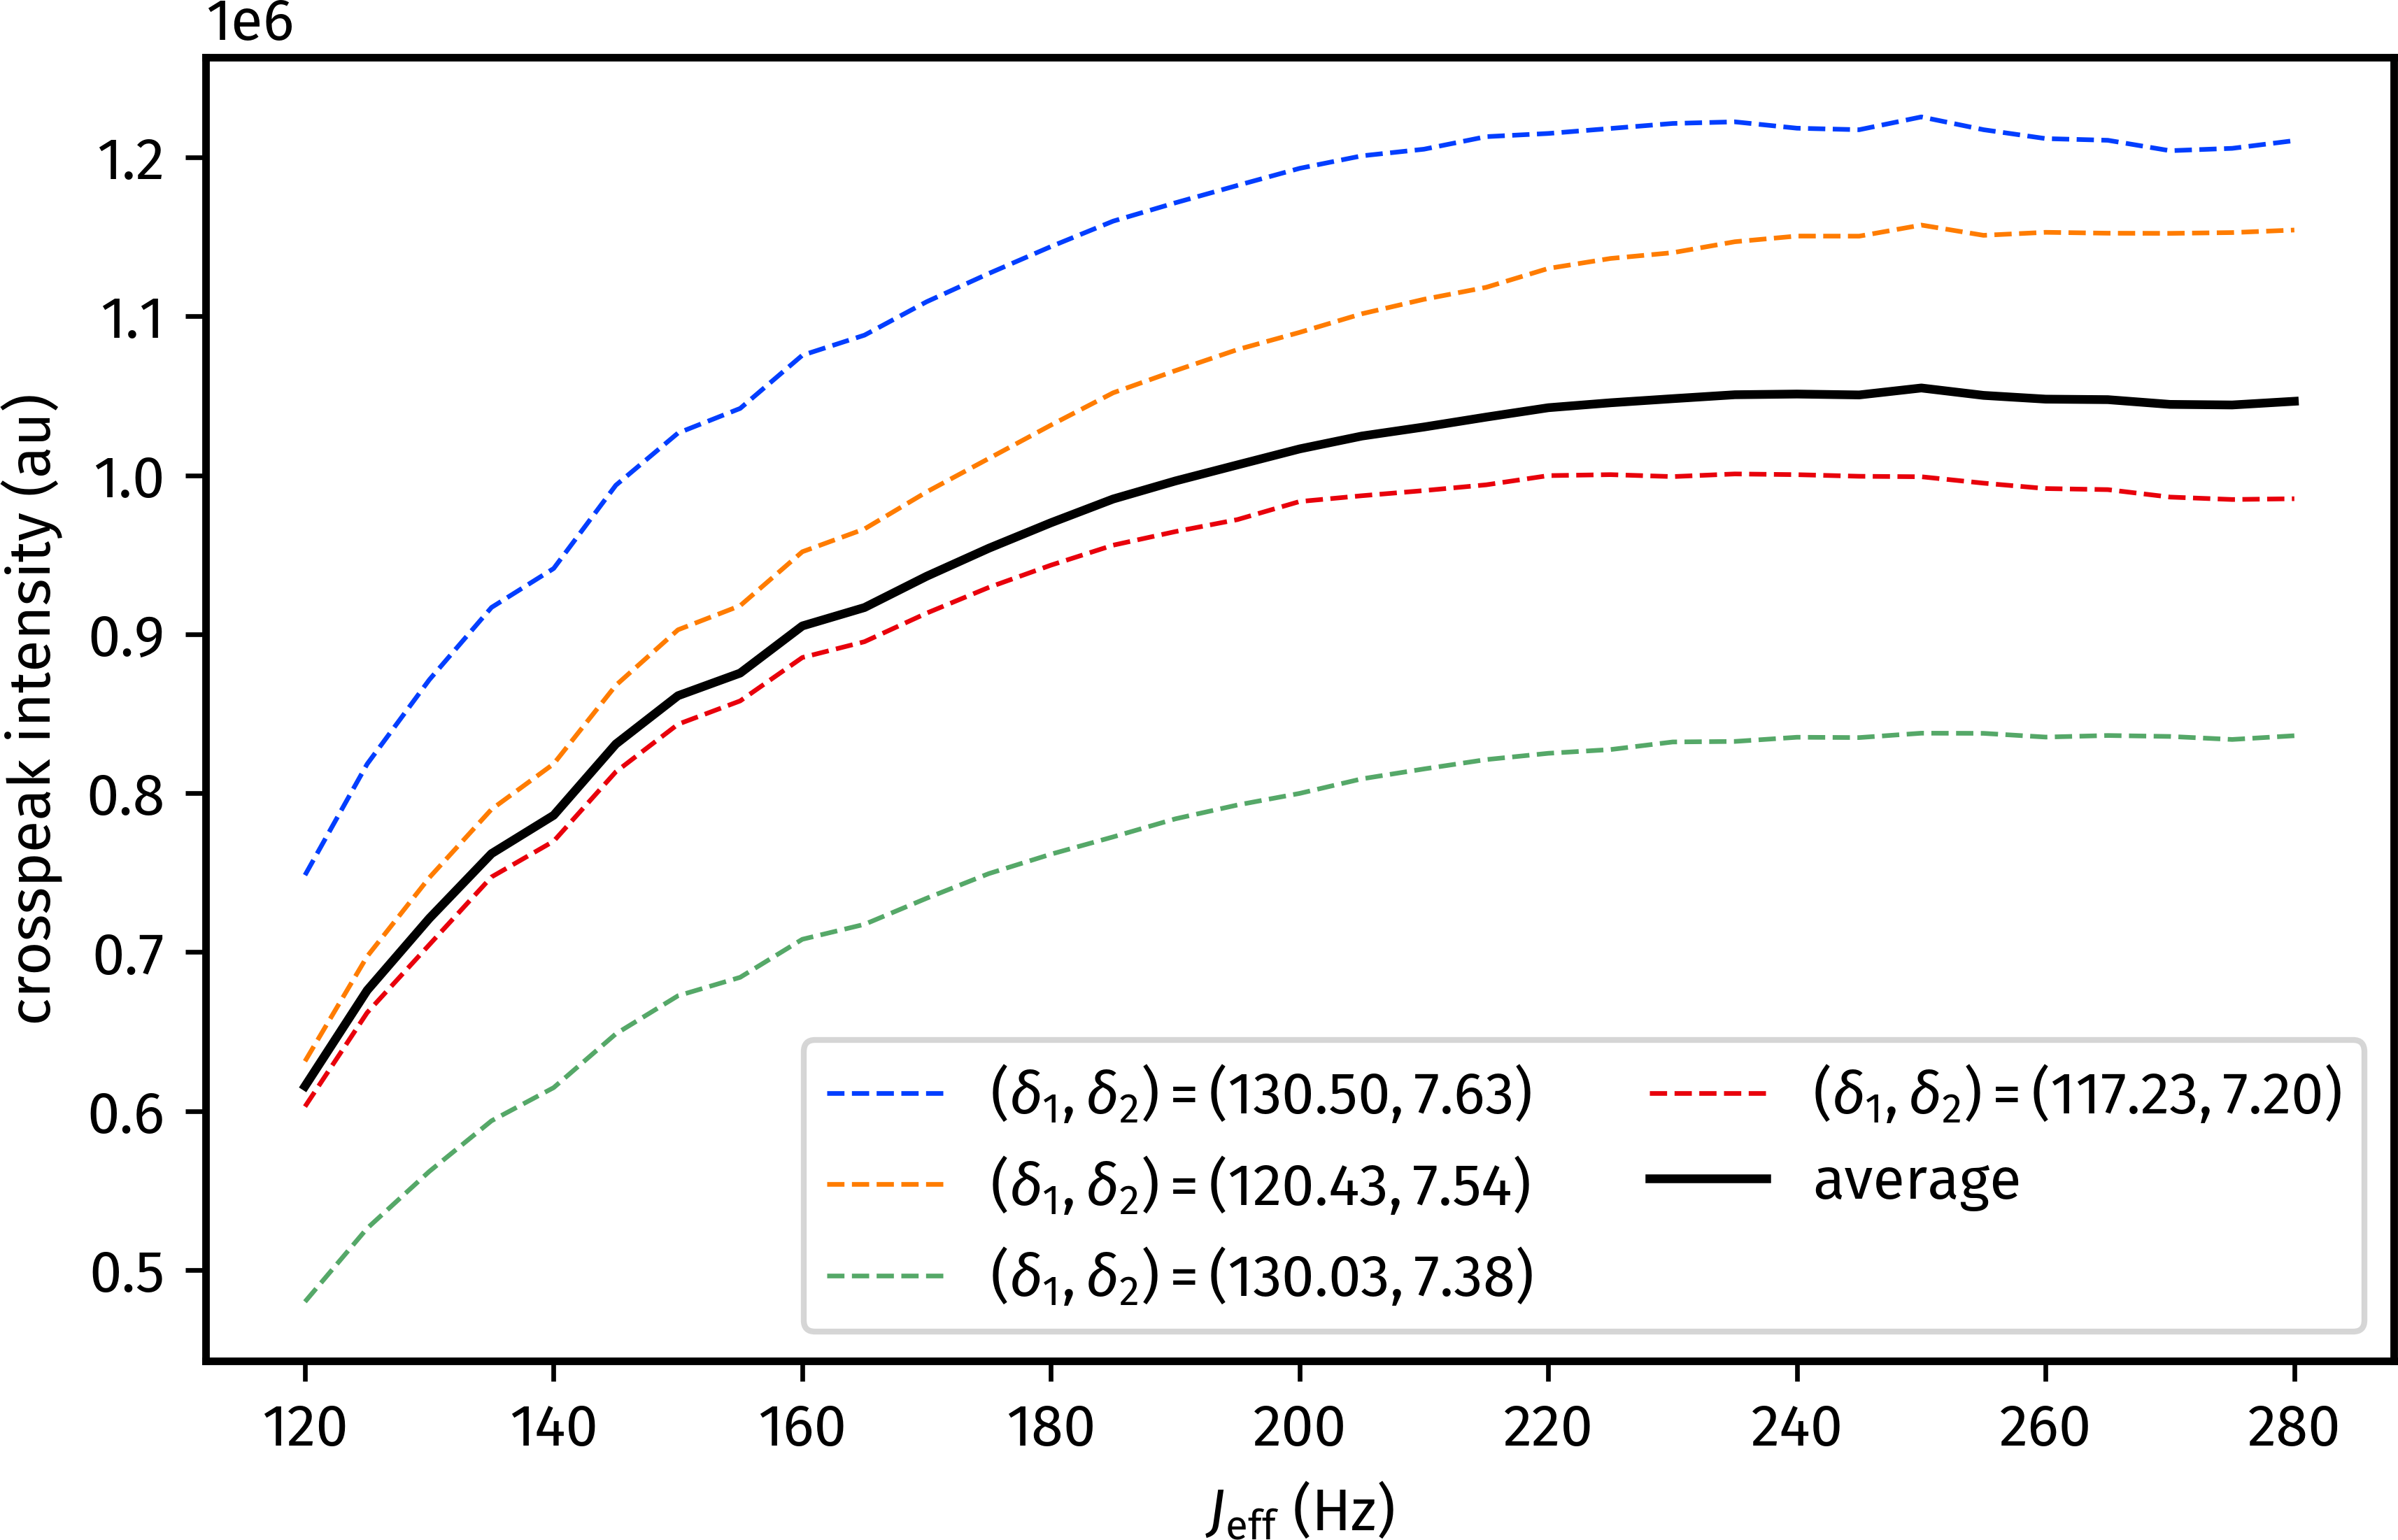
\includegraphics[]{poise/asaphsqc_scan.png}%
    \caption[Reference grid search for ASAP-HSQC excitation delay]{
        Reference grid search showing how the ASAP-HSQC signal intensity for the 3-fluorophenylboronic acid sample varies with $J_\text{eff}$.
        \datacode{7B-200722}
    }
    \label{fig:asaphsqc_scan}
\end{figure}

To speed up the optimisation, optimisations were run using a `low-quality' ASAP-HSQC spectrum with only 32 $t_1$ increments.
A recovery delay of \qty{0.1}{\s} was used.

\subsubsection{Optimisation results}

\begin{table}[htb]
    \hbadness=10000
    \centering
    \begin{tabular}{ccccc}
        \toprule
        Entry & Algorithm & Optimum found (\unit{\Hz}) & FEs  & Time taken (\unit{\s}) \\
        \midrule
        1     & NM        & 250.0--256.3            & 8--9 & 169--195             \\
        2     & MDS       & 237.5--243.8            & 8    & 171--179             \\
        3     & BOBYQA    & 229.8--245.6            & 4--7 & 114--157             \\
        \bottomrule
    \end{tabular}
    \caption[ASAP-HSQC INEPT delay optimisations]{
        ASAP-HSQC INEPT delay optimisations.
        The POISE routine used was: \mintinline[breaklines]{json}{{"name": "asaphsqc", "pars": ["cnst3"], "lb": [120.0], "ub": [280.0], "init": [150.0], "tol": [10.0], "cf": "asaphsqc", "au": "poise_2d"}}.
        \datacode{7B-200722}
    }
    \label{tbl:poise_asaphsqc}
\end{table}

\begin{figure}[htb]
    \centering
    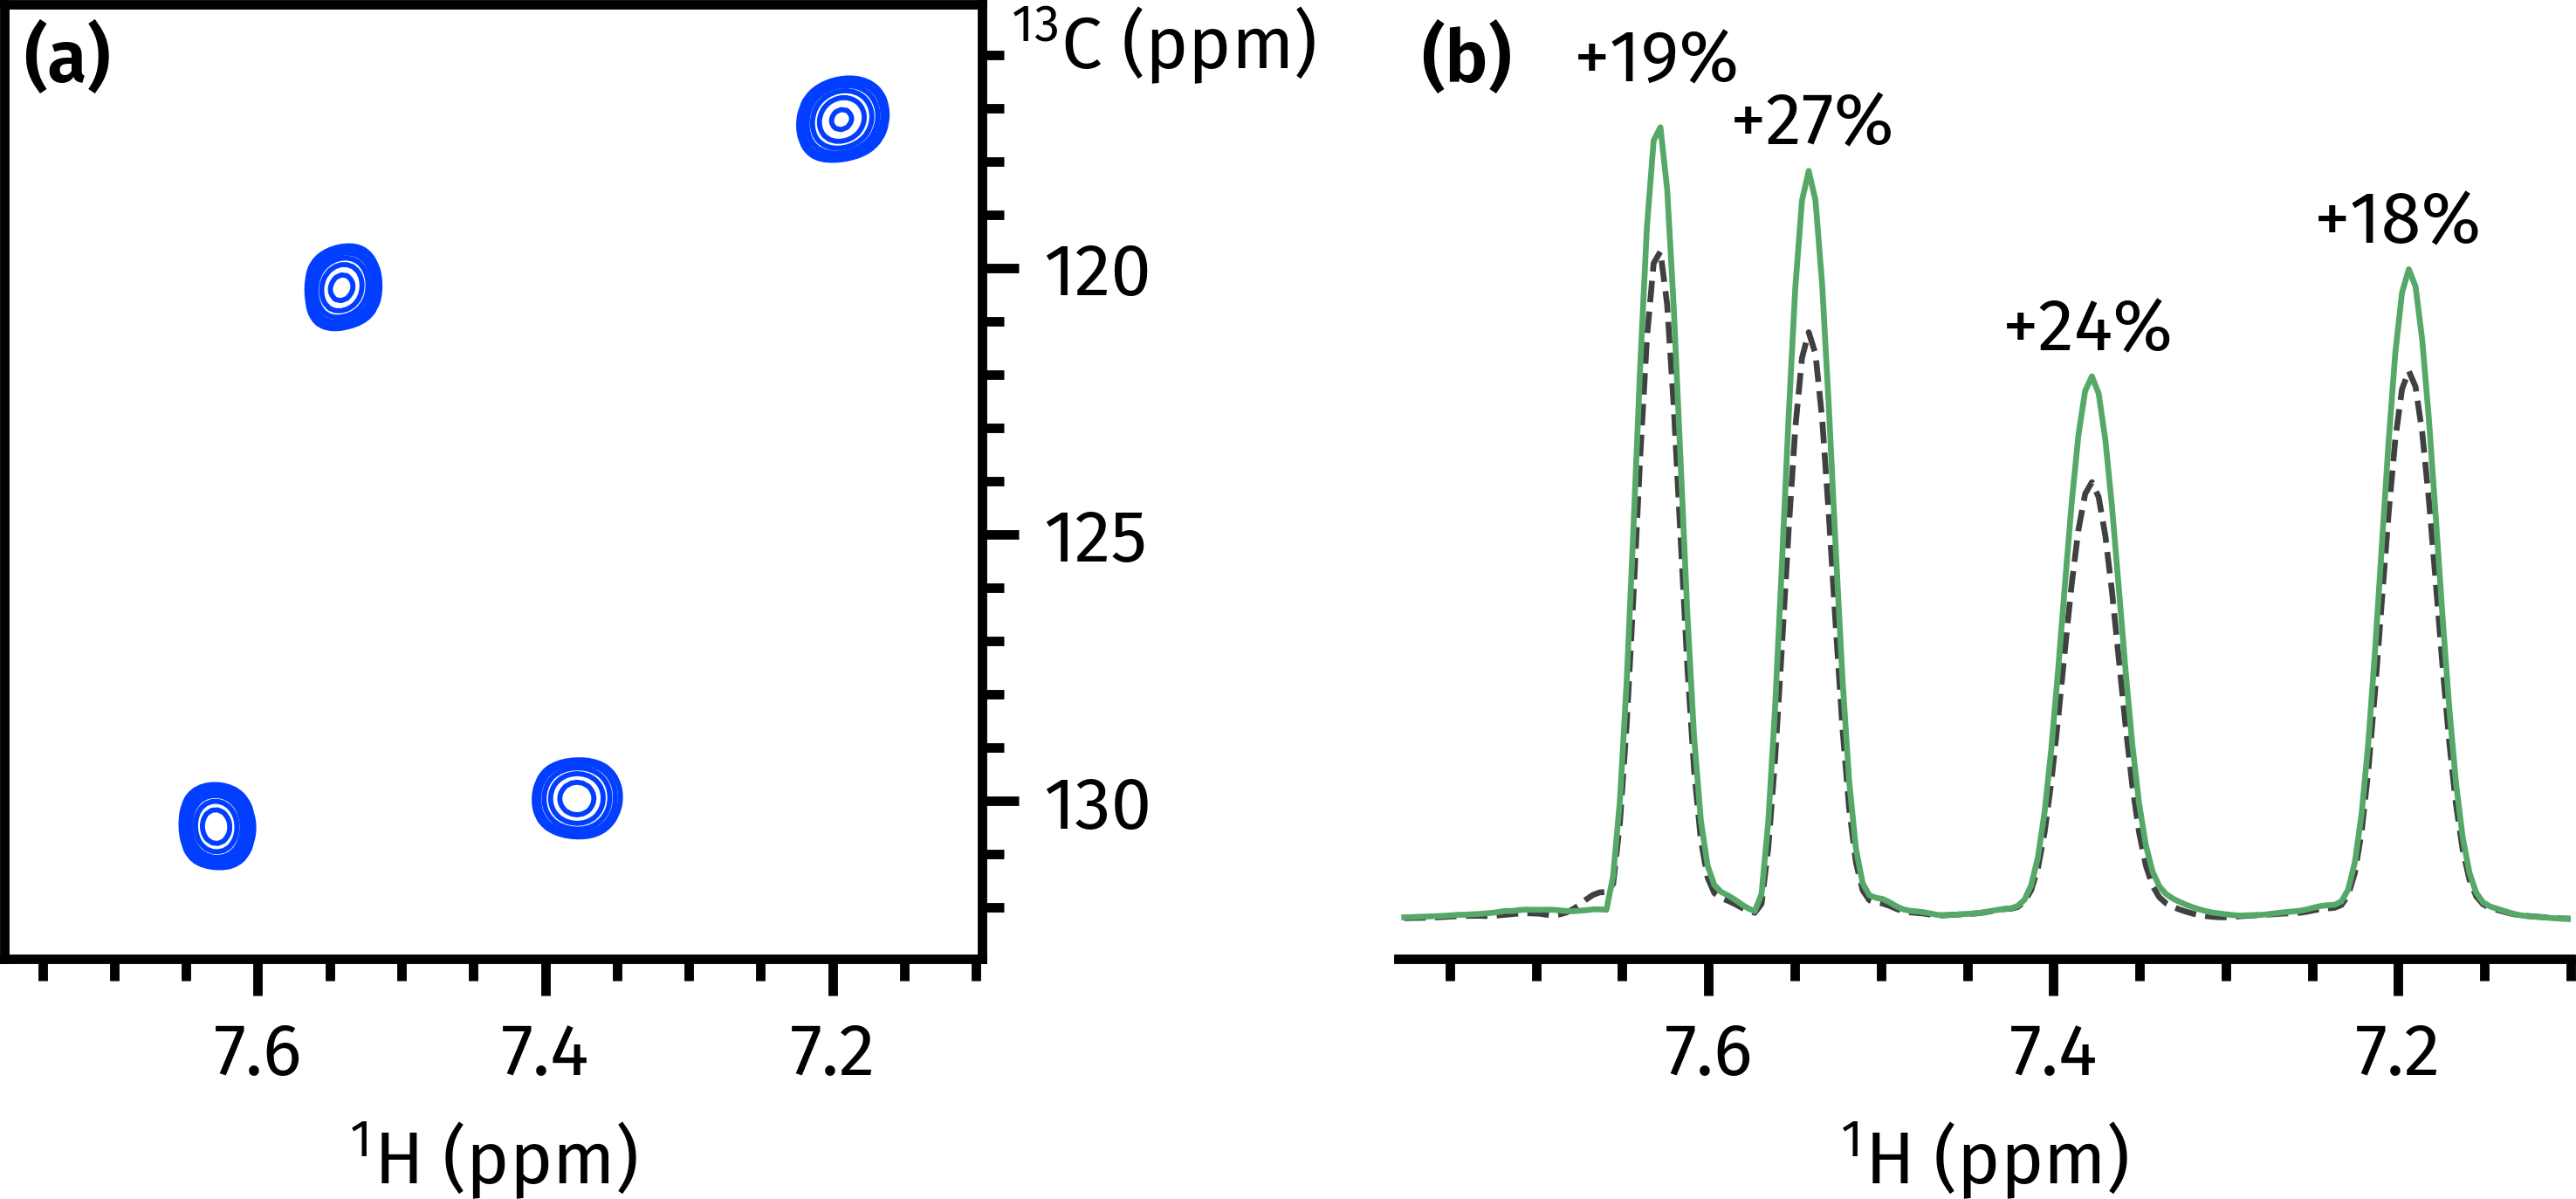
\includegraphics[]{poise/asaphsqc_spec.png}%
    {\phantomsubcaption\label{fig:asaphsqc_spec_spec}}%
    {\phantomsubcaption\label{fig:asaphsqc_spec_proj}}%
    \caption[Projections of ASAP-HSQC spectra before and after optimisation]{
        \textbf{(\subref{fig:asaphsqc_spec_spec})} ASAP-HSQC spectrum of the 3-fluorophenylboronic acid sample.
        \textbf{(\subref{fig:asaphsqc_spec_proj})} Projections of the ASAP-HSQC spectra before (grey dotted line, using $J_\text{eff} = \qty{150}{\Hz}$) and after (green dotted line, using $J_\text{eff} = \qty{245}{\Hz}$) optimisation of the INEPT delay.
        Sensitivity increases for each peak are indicated.
        \datacode{7B-200722}
    }
    \label{fig:asaphsqc_spec}
\end{figure}

The results from the POISE optimisations are collated in \cref{tbl:poise_asaphsqc}.
As can be seen, even though the FE involves acquisition of a 2D spectrum, the optimisation itself completes in just 2--3 minutes, correctly converging to $J_\text{eff}$ values in the region of around \qty{240}{\Hz}.
When re-evaluated on a `full' ASAP-HSQC experiment with 64 $t_1$ increments (\cref{fig:asaphsqc_spec_spec}),%
\footnote{The \carbon{} resonances of interest in this compound fall within a very small window, so relatively few $t_1$ increments are needed.}
the optimisation yielded an 18--27\% improvement in the sensitivity of the ASAP-HSQC spectrum, as shown in \cref{fig:asaphsqc_spec_proj}.
